\section{\large{\textbf{Junkers Ju 248}}}
%========================

\subsection{Początki}


\begin{frame}{\Huge{\textbf{Ju 248 - Początki}}}
	\begin{columns}
		\column{0.5\textwidth} 
			\justifying

W połowie 1944 roku rozpoczęto rozwój \textbf{Ju 248}, bazujący na Messerschmitt Me 163B. Projekt został przeniesiony z Messerschmitta do Junkersa na żądanie RLM, gdyż biuro konstrukcyjne Messerschmitta nie miało już możliwości dalszej pracy. Prof. Hertel zajął się analizą wad Me 163, takich jak krótki czas pracy silnika, słabe osiągi startowe z powodu nart oraz problemy z lądowaniem. \\
W Ju 248 zastosowano skrzydła z Me 163B, ale kadłub został znacząco przeprojektowany. Zamiast nart, nowy model miał chowane podwozie, co poprawiło jego osiągi startowe. Powstały trzy prototypy, z których tylko jeden oblatano w sierpniu 1944 roku; był on ciągnięty przez Me 110 (lub prawdopodobnie Ju 188) bez silników. Planowany był drugi lot na 31 grudnia 1944 roku, jednak dalszy rozwój projektu został przekazany Messerschmittowi jako Me 263 z powodu zakończenia II wojny światowej. 

		\column{0.5\textwidth}
			\begin{figure}
				\centering
				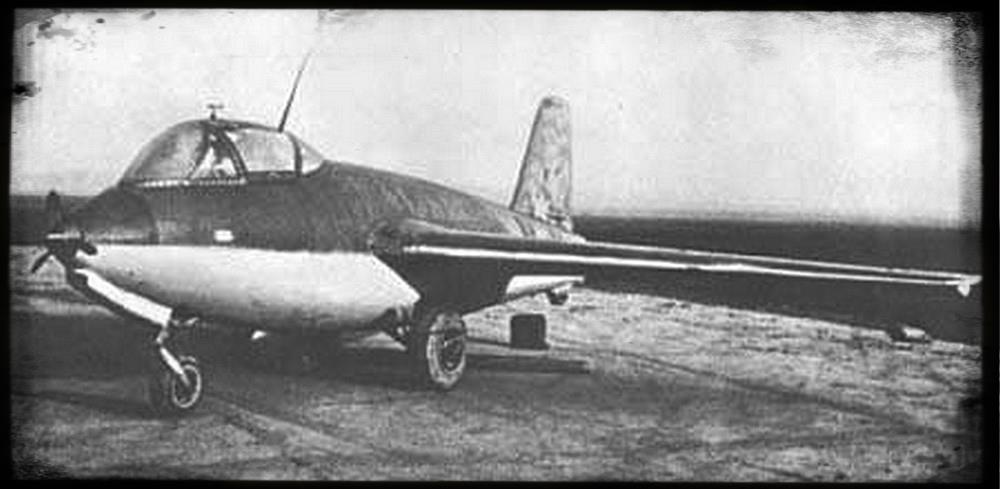
\includegraphics[scale=0.21]{images/ju248-01.jpg}
				\caption{\textit{Ju 248}}
			\end{figure}
	\end{columns}
\end{frame}


%~~~~~~~~~~~~~~~~~~~~~~~~~~~~~~~~~

\subsection{Rozwój}


\begin{frame}{\Huge{\textbf{Ju 248 - Rozwój}}}
	\begin{columns}
		\column{0.47\textwidth} 
			\justifying
			
Prototyp Ju 248 został przechwycony przez Sowietów w Dessau. Schinziger informował, że w Dessau kontynuowano rozwój Ju 248, przeprowadzając testy lotów, podczas których Matthies miał zginąć. Dwa pozostałe prototypy trafiły do Rosji, a niektóre źródła wspominały o wypadku Matthiesa w EF126, co może sugerować pomyłkę w nazwaniu Ju 248. \\
Po wojnie Rosjanie kontynuowali rozwój Ju 248, a niektóre informacje mówią o przeniesieniu jego rozwoju do Siebela w Halle, gdzie już pracowano nad DFS 346. Na podstawie Ju 248 powstał również Mikojan-Gurewicz I-270, który zmienił konstrukcję skrzydła i ogona, ponieważ Rosjanie nie ufali niemieckiemu cofniętemu skrzydłu. Pierwszy lot I-270 odbył się w 1946 roku, ciągnięty przez Tu-2, a z silnikami w 1947 roku. Program I-270 został jednak szybko zakończony z powodu serii katastrof.
			
		\column{0.53\textwidth}
			\begin{figure}
				\centering
				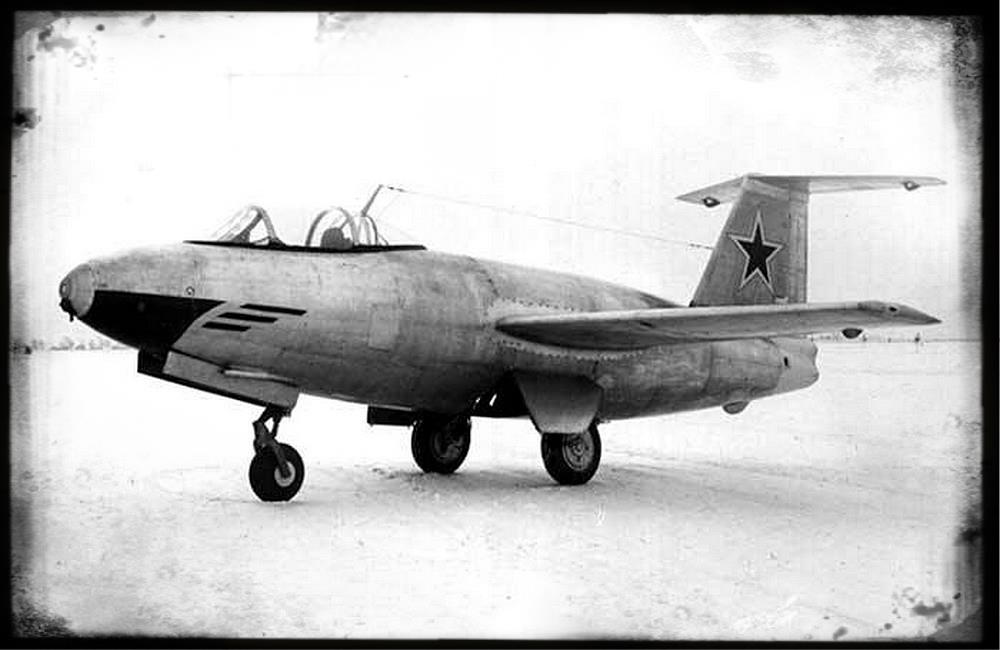
\includegraphics[scale=0.21]{images/ju248-02.jpg}
				\caption{\textit{Ju 248}}
			\end{figure}
	\end{columns}
\end{frame}